\section{Architecture}

This chapter describes the architecture of Stress+.
The whole architecture was designed in a way that arbitrary stress tests can be created with the given modules and new modules can be programmed and added very easily.
Each stress test consist of a pipeline of screens which are show to the patient successively in the specified order.
Additionally a stress test can contain overlays which are displayed on top of the screens.

\begin{figure}[htb]
  \centering
  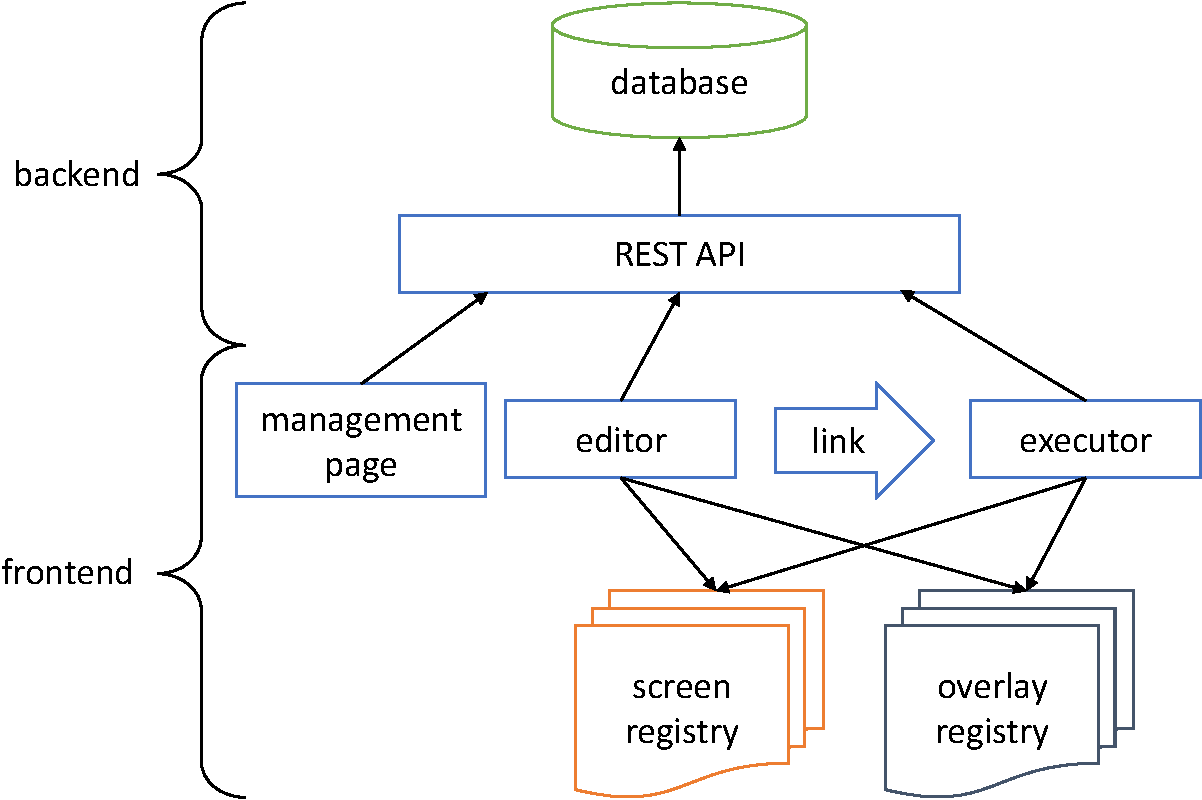
\includegraphics[width=\textwidth]{figures/Architecture-crop}
  \caption{Software architecture}
  \label{fig:software-architecture}
\end{figure}

The figure \ref{fig:software-architecture} shows the software architecture of Stress+, which developed as a browser based application and consists of a frontend and a backend.
The two main frontend components of Stress+ are the \textit{Editor} for creating and editing stress tests and the \textit{Executor} for executing a stress test.
To be able to easily add new modules in the future all availalbe screens and overlays are registered in the \textit{Screen registry} and \textit{Overlay registry}. 
Therefore the \textit{Editor} and \textit{Executor} are developed in a generic way and must query the registries to know which modules are currently present.
After saving a stress test in the \textit{Editor} a link is generated, which can be send to the patient so he can execute the stress test.

The backend is responsible for saving the stress test configurations and the statistics on how the patient performed.
Therefore it consists of a REST API, through which the database can be accessed.

\subsection{Frontend}
The frontend is a Single-page application written in JavaScript with the React framework. 
The following sections describe the different frontend components in more detail

\subsubsection{Screen}
The stress test consists of a list of screens that will be displayed successively to the patient. 
A screen will be displayed fullscreen inside the uses browsers. 
Each screen has its own settings, which can be adjusted inside the editor. 
Screens must be registered in the screen registry to be available.
Following properties must be specified when registering a screen:
\begin{itemize}
  \item The unique name of the screen
  \item The React component for displaying the screen while executing
  \item The React component for displaying the settings of the screen inside the editor
  \item The initial settings of the screen
\end{itemize}

When a screen is displayed during the stress test execution, its React component will receive two properties. 
The \texttt{settings} properties will contain the settings.
The \texttt{onFinished} property is a callback function, which must be called when the current screen is finished and the next screen one should be displayed.

\subsubsection{Overlay}
The stress test can be equipped with overlays that are displayed on top of the current screen. 
All overlays are displayed simultaneously during the whole stress pipeline execution, therefore they do not have an order. 
Each overlay has its own settings, which can be adjusted inside the editor.
For easy positioning of the overlays, an overlay can have the optional property \texttt{position} which controls the position of the overlay on the screen.
Overlays must be registered in the overlay registry to be available.
Following properties must be specified when registering an overlay:
\begin{itemize}
  \item The unique name of the overlay
  \item The React component for displaying the overlay while executing
  \item The React component for displaying the settings of the overlay inside the editor
  \item The initial settings of the overlay
\end{itemize}

When an overlay is displayed during the stress test execution, its React component will receive its settings inside the props.

\subsubsection{Editor}
The stress test can be created and edited in the editor with dragging and dropping items from a toolbar to the pipeline.
The editor has one toolbar for the screens and one for the overlays. 
There are also two separate pipelines for the screens and the overlays. 
Within each item inside a pipeline the user can adjust the settings of the current item. 
Stress test do have a name that can be changed inside the editor.
Each stress test has a unique ID that is generated when it is saved for the first time.
With this ID a link is generated that can be send to patients so they can execute the stress test.
The UI also allows the user to download all statistics for the current stress test.

\subsubsection{Executor}
The executor extracts the unique stress test id from the link and loads the stress test configuration from the backend.
Then the executor will display each screen successively to the patient. 
Screens will receive the settings and a callback function as properties. 
The callback function must be called when the current screen is finished, so the executor can show the next screen. 
All Overlays are displayed simultaneously and each overlay gets their settings as properties.

\subsection{Backend}
The backend consists of the Database and the REST API

\subsubsection{Database}
Because the database should be able to save different stress test configurations and the results of stress test executions the NO-SQL database MongoDB is used.

\subsubsection{REST API}
The REST API is written in JavaScript on the NodeJS platform and uses the express HTTP framework.
